\documentclass[10pt,a4paper,final,oneside,openany,article, twocolumn]{memoir}
% [12pt, 11pt, landscape, titlepage, a4paper, draft, twoside, oneside, 
%  openleft, openright, openany]

\chapterstyle{article}

%BASIC PACKAGES
\usepackage{eso-pic,fix-cm,ae,aecompl,ifthen}         
\usepackage[danish,english]{babel} % last language decides document language!
\usepackage[utf8x]{inputenc}          %text encoding
\usepackage{amsmath,amssymb, amsbsy}  % math
\usepackage{graphicx}
\usepackage[usenames,dvipsnames]{color}
\usepackage[british]{isodate}
%\usepackage{morefloats}
\usepackage[style=alphabetic,natbib=true]{biblatex}
\usepackage{amsmath}
\usepackage[sc]{mathpazo}
\usepackage{MnSymbol}

%\bibliographystyle{apalike}
\bibliography{../bibliography}


\newsubfloat{figure}

%MISC. PACKAGES
%\usepackage{multicol}        % \begin{multicols}{2} \end{multicols}
%\usepackage{array}           % advanced tables
%\usepackage{multirow}        % advanced tables
%\usepackage{longtable}       % split tables over pages
%\usepackage{textcomp}        % symbols
%\usepackage{verbatim}        % monospace code environment
%\usepackage{pdflscape}       % \begin{landscape} \end{landscape}
%\usepackage{semantic}        % Good for proof trees and math ligatures
%\usepackage[noend]{algorithmic}
\usepackage{microtype}        % AWESOME typography!
%\usepackage{colortbl}
%\usepackage{marvosym}
%Kan bruges som \fixme{blabla}. Vises sålænge tex doc er i draft.
\usepackage[draft]{fixme}


%FONT
\usepackage[T1]{fontenc}
\usepackage{palatino}              % font : garamond
\linespread{1.05}                  % Palatino needs more leading (space between lines)
\usepackage{beramono}
%\renewcommand{\ttdefault}{cmtt}    % alternative monospace font
%\renewcommand{\rmdefault}{ugm}
%\usepackage{euler}                % weirdo math
%PAGE DIMENSIONS

%\usepackage[left=4.5cm, right=4.5cm, top=4.4cm, bottom=4.5cm]{geometry}


%HEADERS
\makepagestyle{myheadings}

%\makepsmarks{myheadings}{
%  \def\chaptermark##1{\markboth{%
%    \ifnum \value{secnumdepth} < -1
%      \if@mainmatter
%        \chaptername\ \thechapter\ --- %
%      \fi
%    \fi
%    ##1}{}}

%  \def\sectionmark##1{\markright{%
%    \ifnum \value{secnumdepth} < 0
%      \thesection. \ %
%    \fi
%    ##1}}
%}
%%\makeevenhead{myheadings}{\thechapter\hskip.3cm\vrule\hskip.3cm \leftmark}{}{}
%\makeoddhead{myheadings}{}{}{\leftmark\hskip.3cm\vrule\hskip.3cm\thechapter}
%%\makeoddhead{myheadings}{}{}{\rightmark\hskip.3cm\vrule\hskip.3cm\thesection}
%\makeevenfoot{myheadings}{}{\thepage}{}
%\makeoddfoot{myheadings}{}{\thepage}{}
%\pagestyle{myheadings}

% customize chapter pages

\makepagestyle{myheadingschapterpage}
  \makeevenfoot{myheadingschapterpage}{}{}{\thepage}
  \makeoddfoot{myheadingschapterpage}{}{}{\thepage}
\aliaspagestyle{chapter}{myheadingschapterpage}
\aliaspagestyle{title}{myheadingschapterpage}
\makeevenhead{myheadings}{}{\scshape \thetitle}{}
\makeoddhead{myheadings}{}{\footnotesize\scshape \thetitle}{}
\makeevenfoot{myheadings}{}{}{\thepage}
\makeoddfoot{myheadings}{}{}{\thepage}
\pagestyle{myheadings}



%PDF OUTPUT
\usepackage{hyperref}             % clickable url's in PDF-output
\hypersetup{
%    unicode=true,          % non-Latin characters in Acrobat’s bookmarks
%    pdftitle={My title},    % title
%    pdfauthor={Author},     % author
%    pdfsubject={Subject},   % subject of the document
%    pdfcreator={Creator},   % creator of the document
%    pdfproducer={Producer}, % producer of the document
%    pdfkeywords={keywords}, % list of keywords
%    pdfnewwindow=true,      % links in new window
    colorlinks=true,       % false: boxed links; true: colored links
    linkcolor=black,          % color of internal links
    citecolor=black,        % color of links to bibliography
    filecolor=black,      % color of file links
    urlcolor=black           % color of external links
}




%PRETTY COLORS
\usepackage{color}
\definecolor{blue}{rgb}{0,0,0.8}
\definecolor{green}{rgb}{0,0.5,0}
\definecolor{red}{rgb}{0.5,0,0}
\definecolor{grey}{rgb}{0.5,0.5,0.5}


%SECTION TITLES
\def\thefigure{\arabic{figure}}
%\def\thesection{\arabic{section}}
%\def\thesubsection{\thesection.\arabic{subsection}}
%\def\thesubsubsection{\alph{subsubsection}.}
% \alph \roman \arabin
\setcounter{tocdepth}{1}


% USER DEFINED COMMANDS AND ENVIRONMENTS
%\newcommand{\codevar}[1]{{\tt{\it #1}}}
%\newcommand{\genericleft}{\langle\hspace{-2.6pt}\vert}  % prints [[
%\newcommand{\genericright}{\vert\hspace{-2.6pt}\rangle} % prints ]]
%\newcommand{\generic}[1]{\genericleft #1 \genericright^{\varepsilon}}

%FIGURE CAPTIONS
%\usepackage[labelformat=empty]{subfig}
\usepackage{sidecap} % side captions: \begin{SCfigure}[2.7][ht] ...
\usepackage{caption}
\captionsetup{margin=0pt, font=small, labelfont=bf, format=hang}
\setlength{\abovecaptionskip}{0pt}
\setlength{\belowcaptionskip}{0pt}

%LINE SPACING
%\usepackage{setspace}
%EXAMPLE:
% \singlespacing, \onehalfspacing, \doublespacing, \setstretch{x}


%PROGRAM CODE WITH HIGLIGHTING AND SHAZZ!
%\usepackage{listings}



%DOCUMENT INFO
\title{\vspace{-2cm}
  Fitting an All-atom Protein Model to a $C_\alpha$-trace\\
}
\author{
	Martin Dybdal -- \texttt{dybber@dybber.dk}\\
	Anders Boesen Lindbo Larsen -- \texttt{abll@diku.dk} \\
    Esben Skaarup -- \texttt{sben@sben.dk}
}

%\datebritish
\date{\today}

\newcommand{\subimgwidth}{.48\textwidth}
\newcommand{\imgwidth}{.85\textwidth}
\renewcommand\vec[1]{\boldsymbol{#1}}
\newcommand{\rotateAround}[1]{\lcirclearrowright \hspace{-3mm}\colorbox{white}{}{} \hspace{-1.7mm} _{\scriptscriptstyle #1}}
\setcounter{secnumdepth}{1}
\setcounter{chapter}{0}
%\renewcommand\thesection{\arabic{section}}
\setsecheadstyle{\large\bfseries\raggedright}
\setsubsecheadstyle{\bfseries}

\twocoltocetc
\setlength{\absleftindent}{1.5cm}
\setlength{\absrightindent}{\absleftindent}
			
\begin{document}
\twocolumn[\maketitle
\begin{onecolabstract}
  Protein structure prediction is often simplified by using a model
  that only includes few of the atoms actually present in proteins. In
  particular, the algorithms group at our department only predicts a
  folding of the $C_\alpha$-trace, and are thus excluding most
  backbone atoms and all side-chain molecules.

  In this report we will investigate a strategy for predicting the
  native structure of proteins including all atoms (an all-atom
  model). Our method uses an already folded $C_\alpha$-trace as target.
  \vspace{1.5cm}
\end{onecolabstract}
]
\tableofcontents*

\newpage

\ \\

\hspace{0.5cm}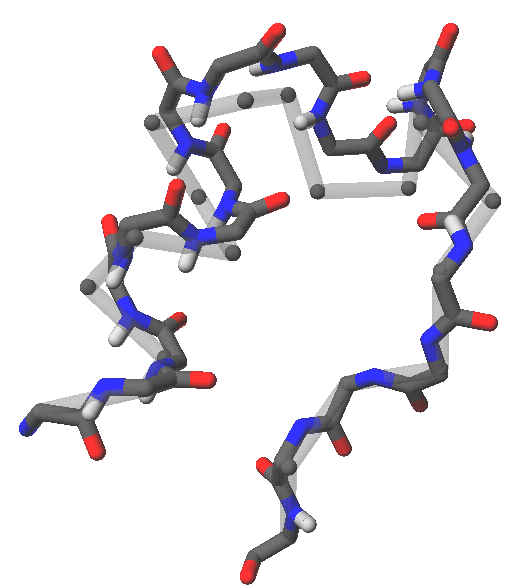
\includegraphics[width=0.4\textwidth]{figures/forside.png}


\newpage
\chapter{Introduction}
Proteins is perhaps the most important molecules of living
organisms. They perform a multitude of biological tasks and is found
in all lifeforms, from bacteria and unicellular organisms to
multicellular organisms such as animals. The chemical abilities and
biological functions of proteins is determined by their
three-dimensional structure. The ability to determine this structure
without performing costly experiments will have many applications in
medicine (e.g. drug design) and biotechnology. Protein structure
prediction and the related topic protein folding\footnote{The two
  research fields are distinguished by whether the actual folding
  process is simulated (protein folding) or a legal structure is
  sought without computing the intermediate steps (protein structure
  prediction).} are large an active research fields. It is still an
open problem.

\section{Protein structure}
The building blocks of proteins are amino acids\footnote{A detailed
  introduction to the structure of proteins is found in
  \cite{branden}}. There are twenty different amino acids which all
share a common structure. The type of amino acid is identified by an
attached molecule called the side-chain. A protein consists of one or
several unbranched chains (polymers) of amino acids. The order of
amino acids in such a chain is the primary structure of the protein.
In Figure \ref{fig:amino_connect} we have shown how a sequence of
amino acids are connected. The carbon atom connecting the backbone
with the side-chains is called the $C_\alpha$-atom.  The largest
variability of the protein structure is found in the angles between
the individual $C_\alpha$-atoms \cite{lotan04}. These angles are
termed $\phi$ and $\psi$ in the literature, Figure \ref{NiceFigure}
illustrates their definition.

% The approach to structure prediction taken by the
% algorithms group at our department is thus to describe the protein
% structure solely by the $C_\alpha$-atoms of the protein
% backbone\fxnote{cite}. Such a sequence of $C_{\alpha}$ atoms is called a
% $C_{\alpha}$-trace (see Figure \ref{fig:Calpha_backbone}).

\subsection{\small TODO}
\begin{itemize}
\item Rotamers
\item Evt. Secondary structure: $\alpha$-helices, $\beta$-sheets (+strands) and loops/turns.
\end{itemize}

\begin{figure}
  \centering
  \subbottom[$C_{\alpha}$-trace]{
    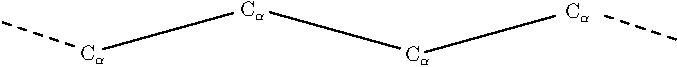
\includegraphics[width=0.48\textwidth]{figures/Calpha_backbone}  
    \label{fig:Calpha_backbone}
  }
  \subbottom[All-atom protein backbone, with $R_1$, $R_2$ and $R_3$ representing side-chains]{
    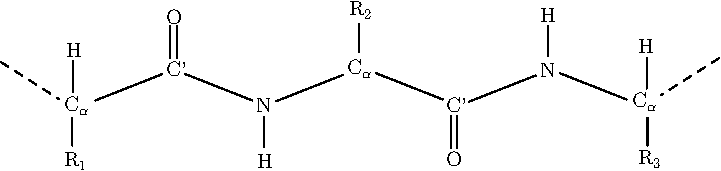
\includegraphics[width=0.48\textwidth]{figures/amino_connect}  
    \label{fig:amino_connect}
  }
  \caption{}
\end{figure}

\section{Protein structure prediction}
The chemical stability of a protein molecule is determined by the
amount of free energy in its structure. It is hypothesized
(\textit{Anfinsens dogma} or the \textit{thermodynamic hypothesis},
\cite{anfinsen73, soundararajan2010}) that all proteins has a unique
stable conformation where the free energy is minimized. This
conformation is known as the native structure of the
protein. Determining it computationally is the problem of protein
structure prediction. Thus, protein structure prediction is an energy
minimization problem.

% Why simplifications are necessary to make the problem
% computationally feasible.

There are generally two approaches to protein structure prediction.
\textit{Comparative modelling} uses information of template proteins
with known native structure and similar amino acid sequences when
performing the prediction. Another approach, known as \textit{ab
  initio} or \textit{de novo} starts ``from scratch'', in the sense
that no information from known structures is used, but instead the
physical/chemical interactions between atoms forms the basis. This
\textit{ab initio} strategy is the approach taken by the algorithms
group at our department.

% Rotamers

\subsection{Evaluating predictions}
%http://cnx.org/content/m11608/latest/
To determine the quality of prediction algorithms it is common \cite{}
to compare predicted structures of a test proteins with the actual
known structure of that protein. The known structure of such test
proteins are obtained by other means (e.g. X-ray Crystallography).
Thus a comparison measure between protein conformations are
needed. The most widely used comparison measure is \textit{least root mean
  square deviation}, lRMSD. RMSD is based on the distances between
corresponding atoms in the two protein conformations under comparison.
If $\vec{A}$ and $\vec{B}$ are two different conformations of the same protein,
where $\vec{a}_i$ and $\vec{b}_i$ are the respective coordinates of atom $i$ in the two
structures, RMSD can be computed by:
\begin{equation}
  \label{eq:rmsd}
  D(\vec{A}, \vec{B}) = \sqrt{\frac{1}{n}\sum_{i=1}^n |\vec{a}_i - \vec{b}_i|^2}
\end{equation}
To compute lRMSD, the RMSD has to be minimized by rotation and
translation of the two conformations. That is, to compute lRMSD, an
\textit{optimal superpositioning} of the conformations is found and
RMSD is computed.


% Limitation: A realistic energy calculation will require an insight in biochemistry
% that is beyond the scope of this project.  Therefore, we limit
% ourselves to minimize the number of clashes as well as the deviation
% from the provided $C_\alpha$-trace.



\section{Our strategy}
In an attempt to get the $C_\alpha$ model closer to the actual
structure of physical proteins, we will in this project try to add the
missing atoms to the protein, to get an all-atom model.  This will
also enable our algorithms group to to participate in the CASP
experiment \cite{caspwebsite}.

The $C_\alpha$-trace generated by their prediction algorithm is used
as target in our fitting of the all-atom model. The fitting should be
conducted, such that it minimizes the number of clashes and at the
same time minimizes the deviation from the target $C_\alpha$-trace.


%%Her vil vi gå igennem vores overordnede strategi:


\section{Related Work}
% SQWRL

\chapter{All-atom Backbone}
Her vil vi forklarer det første trin vi udfører: folder backbonen, med
alle atomer hen til $C_\alpha$-tracet.

$||N - C|| \rotateAround{180^\circ} \rotateAround{90^\circ} \rotateAround{v}$


\section{Inverse kinematics}
Lidt om invers-kinematik.

\chapter{Handling Side-chains}
Hvordan vi tilføjer side-chains og derefter tilpasser hele kæden igen.

\chapter{Evaluation}
Evaluering af metoden med kørsel på diverse kendte proteiner (og
evt. ukendte?)

\chapter{Conclusion}

\defbibheading{bibliography}[\bibname]{%
  \chapter{#1}%
  \markboth{#1}{#1}}
\printbibliography

\end{document}

